%%%%%%%%%%%%%%%%%%%%%%%%%%%%%%%%%%%%%%%%%%%%%%%%%%%%%%%%%%%
%\vspace{-10pt}
%\vspace{\sectionReduceTop}
\section{VQA Dataset Collection}
\label{sec:dataset}
%\vspace{\sectionReduceBot}
%%%%%%%%%%%%%%%%%%%%%%%%%%%%%%%%%%%%%%%%%%%%%%%%%%%%%%%%%%%
\begin{figure*}[t]
\centering
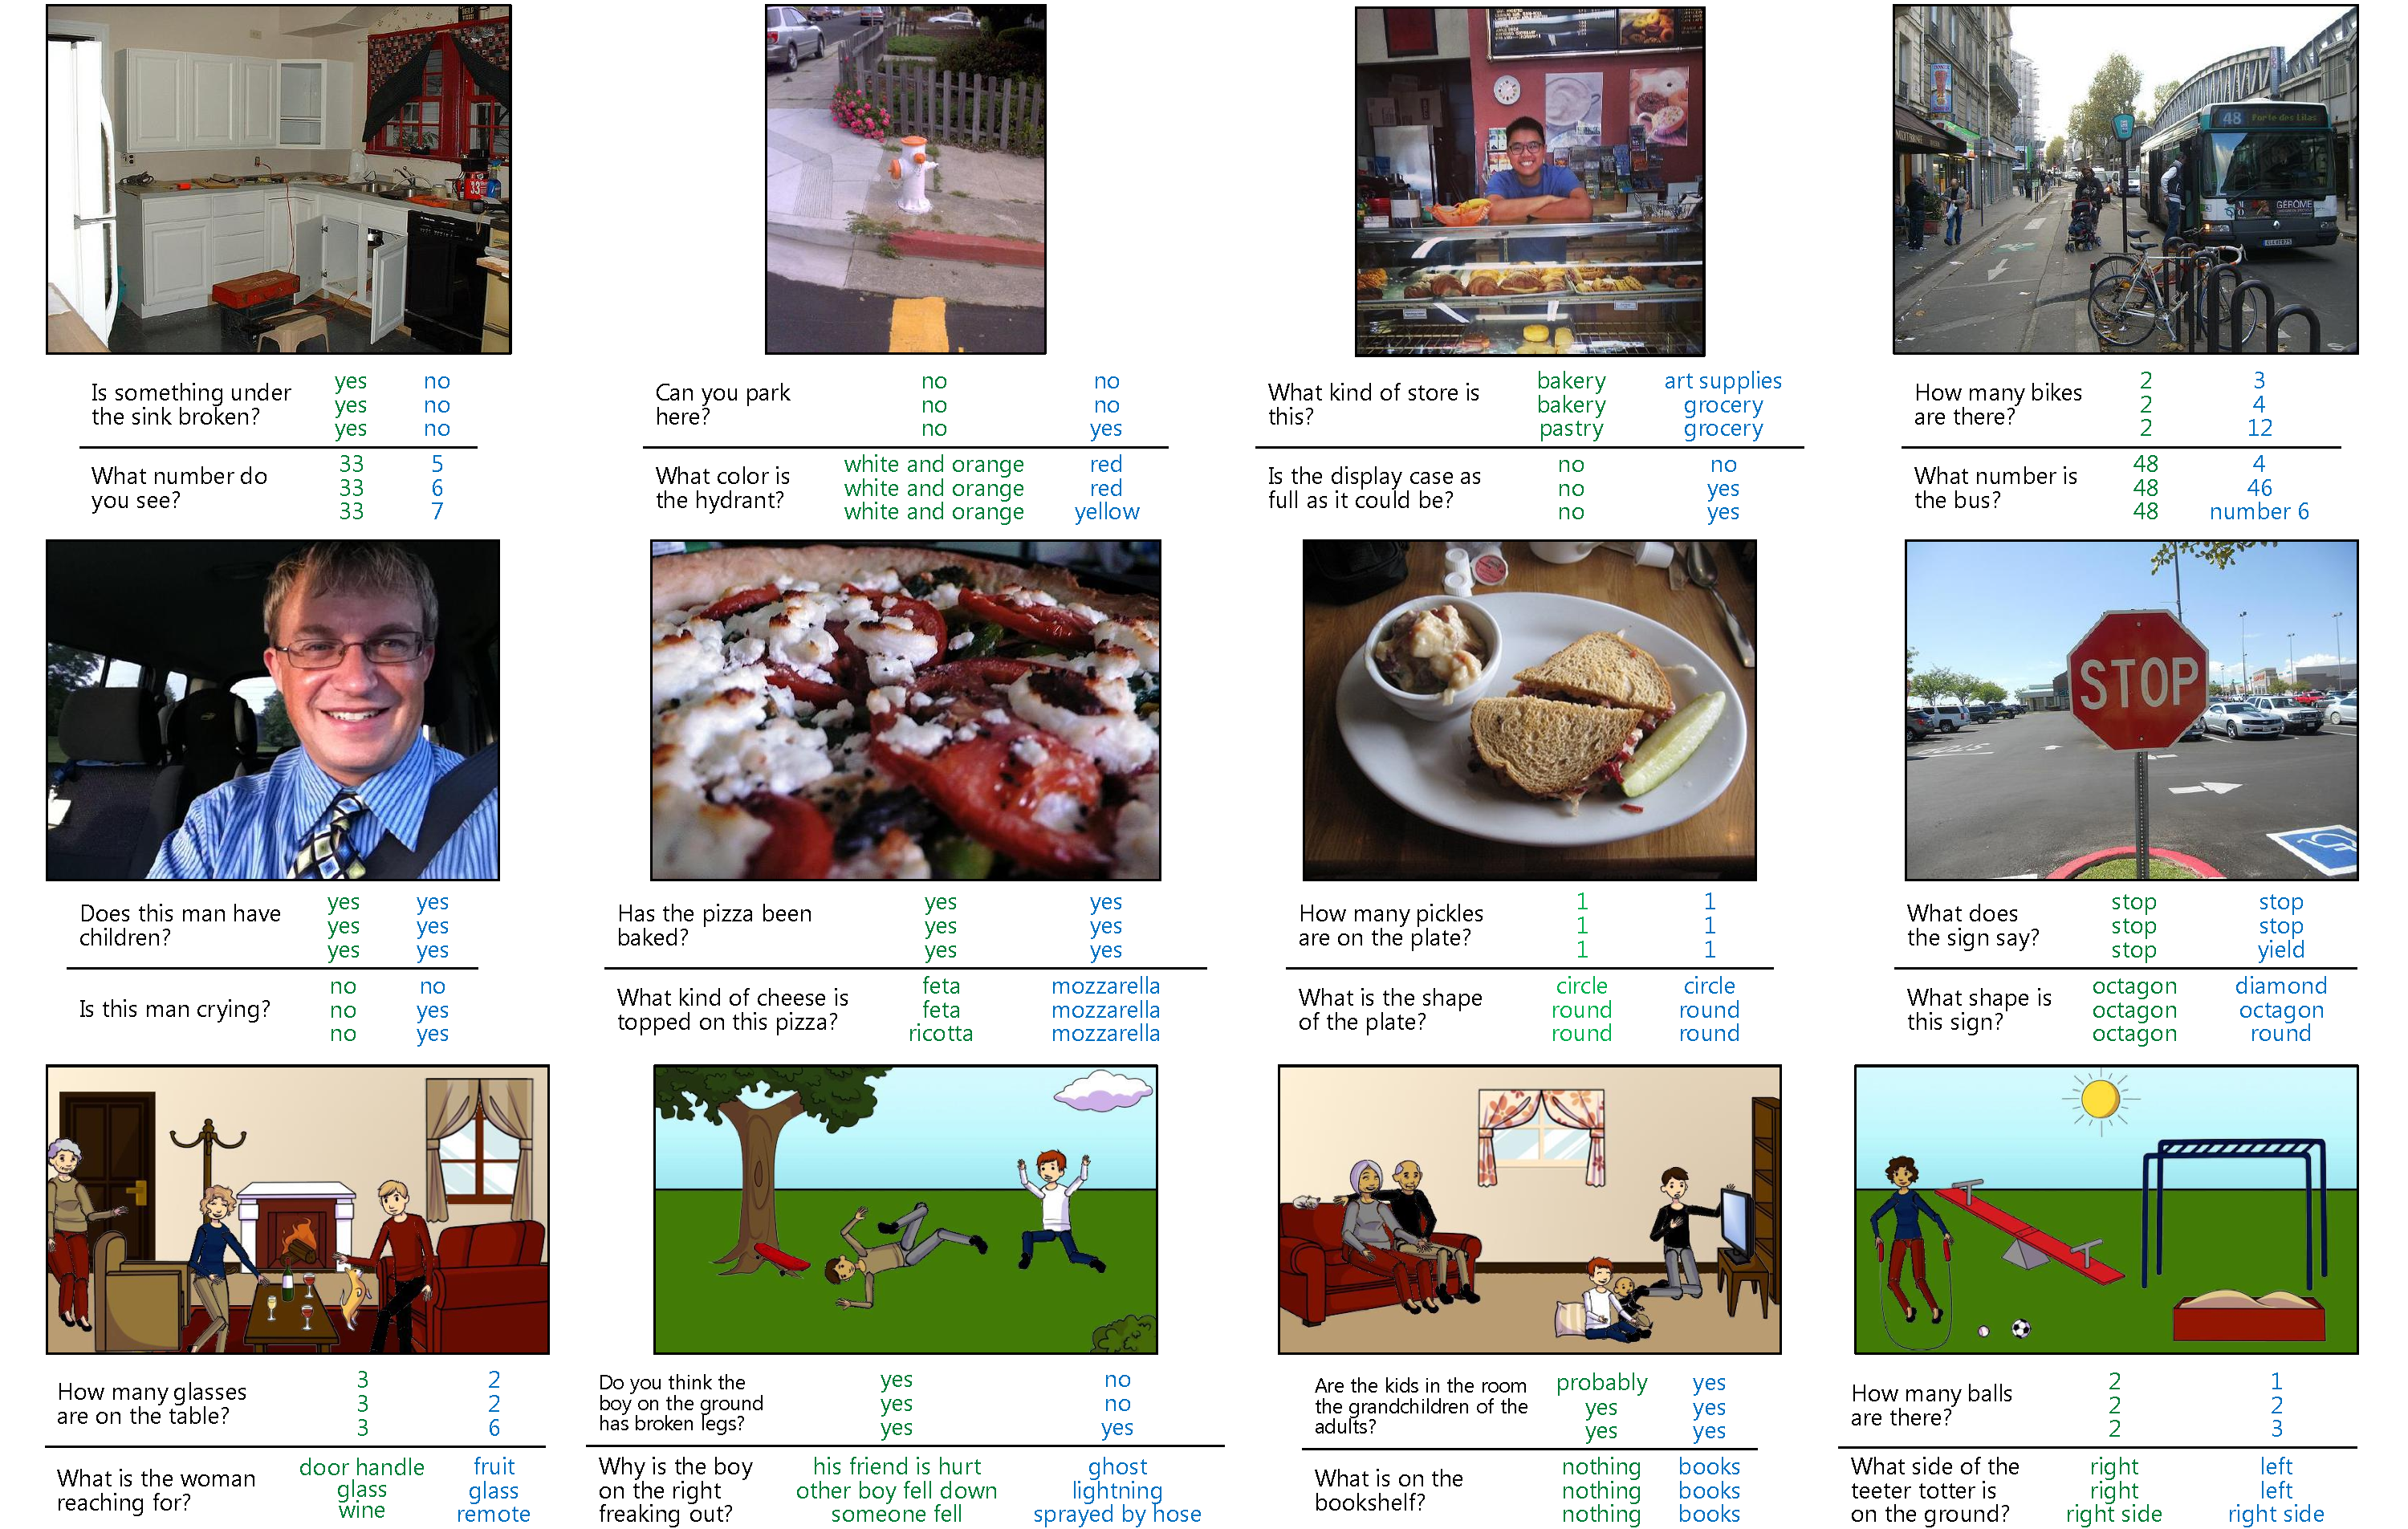
\includegraphics[width=1\linewidth]{figures/figure_02-compressed.pdf}
\caption{Examples of questions (black), (a subset of the) answers given when looking at the image (green), and answers given when not looking at the image (blue) for numerous representative examples of the dataset. See the appendix for more examples.}
%\vspace{-5pt}
\label{fig:qualResults}
%\setlength{\belowcaptionskip}{-10pt}
\end{figure*}
%%%%%%%%%%%%%%%%%%%%%%%%%%%%%%%%%%%%%%%%%%%%%%%%%%%%%%%%%%%
%%%%%%%%%%%%%%%%%%%%%%%%%%%%%%%%%%%%%%%%%%%%%%%%%%%%%%%%%%%
We now describe the Visual Question Answering (VQA) dataset. We begin by
describing the real images and abstract scenes used to collect the questions. Next, we describe
our process of collecting questions and their corresponding answers. Analysis of the questions
and answers gathered as well as baselines' \& methods' results are provided in following sections.

%\vspace{-10pt}
%\paragraph{Real Images:}
\textbf{Real Images.}
%For real images, 
We use the 123,287 training and validation images and 81,434 test images from the newly-released Microsoft
Common Objects in Context (MS COCO)~\cite{coco} dataset. The MS COCO dataset was gathered to find images containing multiple objects and rich contextual information. Given the
visual complexity of these images, they are well-suited for our VQA task. The more diverse our
collection of images, the more diverse, comprehensive, and interesting the resultant set of
questions and their answers.

%\vspace{-10pt}
%\paragraph{Abstract Scenes:}
\textbf{Abstract Scenes.}
The VQA task with real images requires the use of complex and often noisy
visual recognizers. To attract researchers interested in exploring the high-level reasoning
required for VQA, but not the low-level vision tasks, we create a new abstract scenes
dataset \cite{Antol2014,ZitnickCVPR2013,ZitnickICCV2013,VedantamPAMI2015} containing 50K scenes.
The dataset contains 20 ``paperdoll'' human models \cite{Antol2014} spanning genders, races,
and ages with 8 different expressions. The limbs are adjustable to allow
for continuous pose variations. The clipart may be used to depict both
indoor and outdoor scenes. The set contains over 100 objects and 31 animals in
various poses. The use of this clipart enables the creation of more realistic scenes (see bottom row of \figref{fig:qualResults}) that more closely mirror
real images than previous papers \cite{ZitnickCVPR2013,ZitnickICCV2013,VedantamPAMI2015}.
See the appendix
for the user interface, additional details, and examples. 

\textbf{Splits.}
For real images, we follow the same train/val/test split strategy as the MC COCO dataset~\cite{coco} 
(including test-dev, test-standard, test-challenge, test-reserve). For the VQA challenge (see section \ref{sec:challenge}), test-dev is used for debugging and validation experiments and allows for unlimited submission to the evaluation server. Test-standard is the `default' test data for the VQA competition. When comparing to the state of the art (e.g., in papers), results should be reported on test-standard. Test-standard is also used to maintain a public leaderboard that is updated upon submission. Test-reserve is used to protect against possible overfitting. If there are substantial differences between a method's scores on test-standard and test-reserve, this raises a red-flag and prompts further investigation. Results on test-reserve are not publicly revealed. Finally, test-challenge is used to determine the winners of the challenge.

For abstract scenes, we created splits for standardization, separating the scenes into 20K/10K/20K for train/val/test splits, respectively. There are no subsplits (test-dev, test-standard, test-challenge, test-reserve) for abstract scenes.
%For real images, we follow the same \texttt{train}\xspace/\texttt{val}\xspace/\texttt{test}\xspace split strategy as the MC COCO dataset~\cite{coco}. For abstract scenes, we randomly split the scenes into 20K/10K/20K train/val/test splits.}

%\vspace{-10pt}
%\paragraph{Captions.}
\textbf{Captions.}
The MS COCO dataset~\cite{coco,capeval2015} already contains five single-sentence captions for all images.
%Five captions were collected for each image.
%Upon completion, our VQA dataset will contain captions for the abstract scenes using the same user interface\footnote{\url{https://github.com/tylin/coco-ui}} for collection.
We also collected five single-captions for all abstract scenes using the same user interface\footnote{\url{https://github.com/tylin/coco-ui}} for collection.

%\vspace{-10pt}
%\paragraph{Questions:}
\textbf{Questions.}
Collecting interesting, diverse, and well-posed questions is a significant challenge.
Many simple questions may only require low-level computer vision knowledge,
such as ``What color is the cat?'' or ``How many chairs are present in the scene?''.
However, we also want questions that require commonsense knowledge about the scene,
such as ``What sound does the pictured animal make?''. Importantly, questions should also \emph{require} the image to correctly answer and not be answerable using just commonsense information, \eg, in~\figref{fig:teaser}, ``What is the mustache made of?''.  By having a wide variety of
question types and difficulty, we may be able to measure the continual progress of both
visual understanding and commonsense reasoning.

%In our pilot experiments,
We tested and evaluated a number of user interfaces for collecting
such ``interesting'' questions. % and answers.
%Numerous user interfaces were tested and evaluated.
%In order to bias towards ``meaningful'' questions,
%towards those that are more difficult,
Specifically, we ran pilot studies asking human subjects to ask questions about a given image that they believe
a ``toddler'', ``alien'', or ``smart robot'' would have trouble answering.
We found the ``smart robot'' interface to elicit the most interesting and diverse questions. 
%the ``smart robot'' questions were deemed to be
%the most interesting and diverse by the authors.
As shown in the appendix,
our final interface stated:
\begin{center}
\fbox{
\parbox{0.45\textwidth}
{``\emph{We have built a smart robot. It understands a lot about images. It can
recognize and name all the objects, it knows where the objects are, it can recognize the scene
(\eg, kitchen, beach), people's expressions and poses, and properties of objects (\eg, color of
objects, their texture). Your task is to stump this smart robot!}

\emph{Ask a question about this scene that this smart robot probably can not answer, but any human can easily answer while looking at the scene in the image.}''
}
}
\end{center}
To bias against
generic image-independent questions,
%that can be answered using generic commonsense knowledge,
subjects were instructed to ask questions that \emph{require} the image to answer. 

The same user interface was used for both the real images and abstract scenes.
In total, three questions from unique workers were gathered for each image/scene.
When writing a question, the subjects were shown the previous questions already asked for that image to
increase the question diversity. In total, the dataset contains over
$\sim$0.76M questions.


%\vspace{-10pt}
%\paragraph{Answers:}
\textbf{Answers.}
Open-ended questions result in a diverse set of possible answers.
For many questions, a simple ``yes'' or ``no'' response is sufficient. However, other questions
may require a short phrase. Multiple different answers may also be correct. For instance, the
answers ``white'', ``tan'', or ``off-white'' may all be correct answers to the same question.
Human subjects may also disagree on the ``correct'' answer, \eg, some saying ``yes'' while
others say ``no''. To handle these discrepancies, we gather \emph{10 answers for each
question from unique workers}, while also ensuring that the worker answering a question did not ask it.
We ask the subjects to provide answers that are ``a brief phrase and not a complete sentence.
Respond matter-of-factly and avoid using conversational language or inserting your opinion.''
In addition to answering the questions, the subjects were asked ``Do you think you were
able to answer the question correctly?'' and given the choices of ``no'', ``maybe'', and ``yes''. See the appendix for more details about the user interface to collect answers.
See \secref{sec:analysis} for an analysis of the answers provided.

For testing, we offer two modalities for answering the questions: (i) \textbf{open-ended} and (ii) \textbf{multiple-choice}.

For the open-ended task, the generated answers are evaluated %the percentage of
%the human subjects' answers that exactly correspond to the generated answer.
%in a round-robin fashion 
using the following accuracy metric:
%\vspace{-5pt}
\begin{equation*}
\text{accuracy} = \min(\frac{\text{\# humans that provided that answer}}{3},1)
\end{equation*}
%\vspace{-2pt}  
\ie, an answer is deemed 100\% accurate if at least 3 workers provided that exact answer.\footnote{In order 
to be consistent with `human accuracies' reported in \secref{sec:analysis}, machine accuracies are  
averaged over all ${10 \choose 9}$ sets of human annotators}
Before comparison, all responses are made lowercase, numbers converted to digits,
and punctuation \& articles removed. We avoid using soft metrics
such as Word2Vec \cite{word2vec}, since they often group together 
%similar types of 
words that we wish to distinguish, such as ``left'' and ``right''. We also avoid using evaluation metrics from machine translation such as BLEU and ROUGE because such metrics are typically applicable and reliable for sentences containing multiple words. In VQA, most answers (89.32\%) are single word; thus there no high-order n-gram matches between predicted answers and ground-truth answers, and low-order n-gram matches degenerate to exact-string matching. Moreover, these automatic metrics such as BLEU and ROUGE have been found to poorly correlate with human judgement for tasks such as image caption evaluation \cite{DBLP:journals/corr/ChenFLVGDZ15}.

For multiple-choice task, 18 candidate answers are created for each question. As with the open-ended task,
the accuracy of a chosen option is computed based on the number of human subjects who provided 
that answer (divided by 3 and clipped at 1). We generate a candidate set of correct
and incorrect answers from four sets of answers:
%\begin{compactitem}
%\begin{asparaitem}
%\item 
\textbf{Correct:} The most common (out of ten) correct answer.
%\item 
\textbf{Plausible:} To generate incorrect, but still plausible answers we ask
three subjects to answer the questions without seeing the image. See the appendix for more details about the user interface to collect these answers. If three unique answers
are not found, we gather additional answers from nearest neighbor questions
using a bag-of-words model. The use of these answers helps ensure the image,
and not just commonsense knowledge, is necessary to answer the question.
%\item 
\textbf{Popular:} These are the 10 most popular answers. For instance, these are ``yes'',
``no'', ``2'', ``1'', ``white'', ``3'', ``red'', ``blue'', ``4'', ``green'' for real images.
%and ``yes'', ``no'', ``2'', ``1'', ``red'', ``3'', ``white'', ``4'', ``blue'', ``yellow'' for abstract images.}
The inclusion of the most popular answers makes it more difficult for algorithms to infer the type of
question from the set of answers provided, \ie, learning that it is a ``yes or no'' question just because
``yes'' and ``no'' are present in the answers.
%\item 
\textbf{Random:} Correct answers from random questions in the dataset.
%Random answers from other questions. 
To generate a total of 18 candidate answers, we first find the union of the correct, plausible, and popular answers. 
We include random answers until 18 unique answers are found.
%\end{compactitem}
%\end{asparaitem}
The order of the answers is randomized. Example multiple choice questions are in the appendix.

Note that all 18 candidate answers are unique. But since 10 different subjects answered every question, it is possible that more than one of those 10 answers be present in the 18 choices. In such cases, according to the accuracy metric, multiple options could have a non-zero accuracy.